
% --------------------------------------------------------------
% This is all preamble stuff that you don't have to worry about.
% Head down to where it says "Start here"
% --------------------------------------------------------------

\documentclass[10pt]{article}

\usepackage[margin=.7in]{geometry}
\usepackage{amsmath,amsthm,amssymb,mathrsfs}
\usepackage{enumitem}
\usepackage{tikz-cd}
\usepackage{mathtools}
\usepackage{amsfonts}
\usepackage{listings}
\usepackage{algorithm2e}
\usepackage{verse,stmaryrd}
\usepackage{fancyvrb}

% Number systems
\newcommand{\NN}{\mathbb{N}}
\newcommand{\ZZ}{\mathbb{Z}}
\newcommand{\QQ}{\mathbb{Q}}
\newcommand{\RR}{\mathbb{R}}
\newcommand{\CC}{\mathbb{C}}
\newcommand{\PP}{\mathbb P}
\newcommand{\FF}{\mathbb F}
\newcommand{\DD}{\mathbb D}
\renewcommand{\epsilon}{\varepsilon}

\newcommand{\Aut}{\operatorname{Aut}}
\newcommand{\coker}{\operatorname{coker}}
\newcommand{\CVect}{\CC\operatorname{-Vect}}
\newcommand{\Cantor}{\mathcal{C}}
\newcommand{\D}{\mathcal{D}}
\newcommand{\card}{\operatorname{card}}
\newcommand{\dbar}{\overline \partial}
\DeclareMathOperator*{\esssup}{ess\,sup}
\newcommand{\GL}{\operatorname{GL}}
\newcommand{\Hom}{\operatorname{Hom}}
\newcommand{\id}{\operatorname{id}}
\newcommand{\Ind}{\operatorname{Ind}}
\newcommand{\Inn}{\operatorname{Inn}}
\newcommand{\interior}{\operatorname{int}}
\newcommand{\lcm}{\operatorname{lcm}}
\newcommand{\mesh}{\operatorname{mesh}}
\newcommand{\LL}{\mathcal L_0}
\newcommand{\Leb}{\mathcal{L}_{\text{loc}}^2}
\newcommand{\Lip}{\operatorname{Lip}}
\newcommand{\ppGL}{\operatorname{PGL}}
\newcommand{\ppic}{\vspace{35mm}}
\newcommand{\ppset}{\mathcal{P}}
\DeclareMathOperator{\proj}{proj}
\DeclareMathOperator*{\Res}{Res}
\newcommand{\Riem}{\mathcal{R}}
\newcommand{\RVect}{\RR\operatorname{-Vect}}
\newcommand{\Sch}{\mathcal{S}}
\newcommand{\SL}{\operatorname{SL}}
\newcommand{\sgn}{\operatorname{sgn}}
\newcommand{\spn}{\operatorname{span}}
\newcommand{\Spec}{\operatorname{Spec}}
\newcommand{\supp}{\operatorname{supp}}
\newcommand{\Torus}{\mathbb T}
\DeclareMathOperator{\tr}{tr}

\DeclareMathOperator{\adj}{adj}
\DeclareMathOperator{\curl}{curl}

% Calculus of variations
\DeclareMathOperator{\pp}{\mathbf p}
\DeclareMathOperator{\zz}{\mathbf z}
\DeclareMathOperator{\uu}{\mathbf u}
\DeclareMathOperator{\vv}{\mathbf v}
\DeclareMathOperator{\ww}{\mathbf w}

\DeclareMathOperator{\Olo}{\mathscr O}

% Categories
\newcommand{\Ab}{\mathbf{Ab}}
\newcommand{\Cat}{\mathbf{Cat}}
\newcommand{\Group}{\mathbf{Group}}
\newcommand{\Module}{\mathbf{Module}}
\newcommand{\Set}{\mathbf{Set}}
\DeclareMathOperator{\Fun}{Fun}
\DeclareMathOperator{\Iso}{Iso}

% Complex analysis
\renewcommand{\Re}{\operatorname{Re}}
\renewcommand{\Im}{\operatorname{Im}}

% Logic
\renewcommand{\iff}{\leftrightarrow}
\newcommand{\Henkin}{\operatorname{Henk}}
\newcommand{\PA}{\mathbf{PA}}
\DeclareMathOperator{\proves}{\vdash}

% Group
\DeclareMathOperator{\Gal}{Gal}
\DeclareMathOperator{\Fix}{Fix}
\DeclareMathOperator{\Out}{Out}

% Other symbols
\newcommand{\heart}{\ensuremath\heartsuit}

\DeclareMathOperator{\atanh}{atanh}

% Theorems
\theoremstyle{definition}
\newtheorem*{corollary}{Corollary}
\newtheorem*{falselemma}{Grader's ``Lemma"}
\newtheorem{exer}{Exercise}
\newtheorem{lemma}{Lemma}[exer]
\newtheorem{theorem}[lemma]{Theorem}

\usepackage[backend=bibtex,style=alphabetic,maxcitenames=50,maxnames=50]{biblatex}
\renewbibmacro{in:}{}
\DeclareFieldFormat{pages}{#1}

\begin{document}
\noindent
\large\textbf{Finite element methods, HW 1} \hfill \textbf{Aidan Backus} \\
% --------------------------------------------------------------
%                         Start here
% --------------------------------------------------------------\

\begin{exer}
    Let $J$ denote the Plateau energy. Suppose that $u$ is a minimizer, and show that $u$ satisfies the variational equation 
\begin{equation}\label{Variational}
    \int_\Omega \frac{\nabla u \cdot \nabla v}{\sqrt{1 + |\nabla u|^2}} ~dx = 0.
\end{equation}
\end{exer}

By a coincidence (or is it that much of a coincidence? It's practically \emph{the} central example in variational calculus) I'm currently writing a paper about the Plateau equation!
And I use the fact that you can approximate it by the Poisson equation quite often...

Anyways, we suppose that $v \in V$ is a test function and $\varepsilon$ is a small parameter. Then
$$J(u + \varepsilon v) = \int_\Omega \sqrt{1 + |\nabla u|^2 + 2\varepsilon \nabla u \cdot \nabla v + \varepsilon^2 |\nabla v|^2} ~dx.$$
Using the expansion 
\begin{equation}\label{Taylor sqrt}
    \sqrt{1 + a + b} - \sqrt{1 - a} = \frac{b}{2\sqrt{1 + a}} + O(b^2)
\end{equation}
valid in the limit $b \to 0$, we have 
$$J(u + \varepsilon v) - J(u) = \int_\Omega \frac{2\varepsilon \nabla u \cdot \nabla v + \varepsilon^2 |\nabla v|^2}{2\sqrt{1 + |\nabla u|^2}} + O(\varepsilon^2) ~dx.$$
But the term $\varepsilon |\nabla v|^2/\sqrt{1 + |\nabla u|^2}$ is also $O(\varepsilon^2)$ so (approximating $v$ by a function in $C^\infty_c(V)$ to ensure that all integrals are finite and go to $0$ as $\varepsilon \to 0$; we omit the uninteresting details),
$$J(u + \varepsilon v) - J(u) = \varepsilon \int_\Omega \frac{\nabla u \cdot \nabla v}{\sqrt{1 + |\nabla u|^2}} + O(\varepsilon^2).$$
Dividing both sides by $\varepsilon$ and taking $\varepsilon \to 0$, we obtain the first variation of $J$,
$$\partial_v J(u) = \int_\Omega \frac{\nabla u \cdot \nabla v}{\sqrt{1 + |\nabla u|^2}},$$
but $u$ is a minimizer in the same admissible class as $v$, so $\partial_v J = 0$.

\begin{exer}
    Show that if $u$ is smooth enough then $u$ solves the equation 
\begin{equation}\label{MSE}
    -\nabla \cdot \left(\frac{\nabla u}{\sqrt{1 + |\nabla u|^2}}\right) = 0.
\end{equation}
\end{exer}

If $u$ is twice-differentiable, then we can integrate (\ref{Variational}) by parts to remove the derivative from the $v$.
Since $v$ is trace-free, there is no boundary term and we obtain 
$$-\int_\Omega \nabla \cdot \left(\frac{\nabla u}{\sqrt{1 + |\nabla u|^2}}\right) v ~dx = 0.$$
From the Lebesgue differentiation theorem we immediately see that (\ref{MSE}) holds almost everywhere.
If furthermore $u \in C^2$ then $-\nabla \cdot(\nabla u/\sqrt{1 + |\nabla u|^2})$ is continuous and so the only way that it can annihilate every test function is if it is $0$ everywhere. 

\begin{exer}
    Show that $u$ solves the Plateau equation 
\begin{equation}\label{Plateau}
    u_{xx}(1 + u_y^2) - 2u_{xy} u_x u_y + u_{yy}(1 + u_x^2) = 0.
\end{equation}
\end{exer}

From the quotient rule and (\ref{MSE}),
\begin{align*}
0 &= -\nabla \cdot \frac{\nabla u}{\sqrt{1 + |\nabla u|^2}} \\
&= -\partial_x \frac{u_x}{\sqrt{1 + u_x^2 + u_y^2}} - \partial_y \frac{u_y}{\sqrt{1 + u_x^2 + u_y^2}} \\
&= \frac{u_x u_y u_{xy} - u_{xx} (1 + u_y^2)}{(1 + u_x^2 + u_y^2)^{3/2}} + \frac{u_x u_y u_{xy} - u_{yy}(1 + u_x^2)}{(1 + u_x^2 + u_y^2)^{3/2}}.
\end{align*}
Multiplying both sides by $-(1 + u_x^2 + u_y^2)^{3/2}$, which is never zero, we obtain (\ref{Plateau}).

\begin{exer}
    Show that $u = a + bx + cy$ solves Plateau's equation. Explain why this is true physically.
\end{exer}

We derived the Plateau energy $J(u)$ as the surface area of the graph of $u$.
It is not surprising that $u$ minimizes this quantity for some boundary data, because a plane minimizes area, and the graph of $u$ is a plane.
Indeed, $u_{xx} = b_x = 0$, $u_{yy} = c_y = 0$, and $u_{xy} = b_y + c_x = 0$, so plugging all these terms into Plateau's equation we see that $u$ solves Plateau's equation.

\begin{exer}
    Show that $u = \cosh^{-1} r$ solves Plateau's equation. Sketch the solution. How is this a soap film?
\end{exer}

Let us show that the surface $z = u(r)$, in cylindrical coordinates
$$(r, \theta, z) \in \RR_+ \times S^1 \times I,$$
has minimal surface area, where $I \subseteq \RR$ is an interval. If this is true, then $u$ will minimize $J$ and hence solve Plateau's equation.
Minimization of area is a local property and so we can extend $z = u(r)$ to the surface of revolution
$$E = \{(r, \theta, z) \in \RR_+ \times S^1 \times I: r = \cosh z\}.$$
If we fix $\theta_0 \in S^1$ and define
$$\gamma(z) = (\cosh z, \theta_0, z),$$
and let $ds^2 = dr^2 + dz^2$ denote the metric on $\gamma$, then because $E$ is a surface of revolution, its surface area is
$$|E| = \int_\gamma 2\pi r ~ds = 2\pi \int_I \cosh z \sqrt{1 + \sinh^2 z} ~dz.$$
Let $F$ be a competitor to $E$ in the set $\RR_+ \times S^1 \times I$. Then, since $F$ is a competitor, we have an equality of boundary values
$$E \cap (\RR_+ \times S^1 \times \partial I)  = F \cap (\RR_+ \times S^1 \times \partial I).$$
Since the boundary value of $F$ consists of a circle on each connected component of $\RR_+ \times S^1 \times \partial I$, if $F$ is to be a minimizer, then $F$ must be a surface of revolution.
Therefore we may restrict to competitors which are themselves surfaces of revolution and hence there exists a function $F: I \to \RR$ such that 
$$|F| = 2\pi \int_I \sqrt{1 + F'(z)^2} ~dz.$$
So it remains to show that $\cosh$ is a minimizer of the Lagrangian 
$$\mathscr L[f] = \int_I f(z) \sqrt{1 + f'(z)^2} ~dz.$$
(This Lagrangian is somewhat nicer than the Plateau energy $J$, since its domain of integration is an interval rather than a surface.)
If $g$ is a competitor to $f$ and $\varepsilon$ is a small parameter, then 
\begin{align*}
    \mathscr L[f + \varepsilon g] &= \int_I f(z) \sqrt{1 + f'(z)^2 + \varepsilon f'(z) g'(z) + \varepsilon^2 g'(z)^2} \\
    &\qquad + \varepsilon g(z) \sqrt{1 + f'(z)^2 + \varepsilon f'(z) g'(z) + \varepsilon^2 g'(z)^2} ~dz \\
    &= \mathscr L[f] + \varepsilon \int_I \frac{f'(z) g'(z)}{\sqrt{1 + f'(z)^2}} ~dz + \varepsilon \int_I g(z) + \sqrt{1 + f'(z)^2} ~dz + O(\varepsilon^2)
\end{align*}
by (\ref{Taylor sqrt}). Taking $\varepsilon \to 0$ we conclude that $f$ is a minimizer exactly when 
$$0 = \int_I \frac{f'(z) g'(z)}{\sqrt{1 + f'(z)^2}} f(z) + \sqrt{1 + f'(z)^2} g(z) ~dz.$$
But if $f(z) = \cosh z$ then $f(z) = \sqrt{1 + f'(z)^2}$, so it suffices to show 
$$0 = \int_I \sinh z g'(z) + \cosh z g(z) ~dz.$$
This is immediate from integration by parts and the fact that $\sinh' z = \cosh z$.

The connection with soap films is apparent when we consider the full surface of revolution $E$. Its boundary $E' = E \cap (\RR_+ \times S^1 \times \partial I)$ consists of two circles, which one can think of as edges of the soap film, say the beginning and end points of the trajectory of a soap wand.
One intuitively expects the soap film created during the motion of the wand to minimize area between those two circles, and therefore must be $E$.
Here is a crude picture of what such a film would look like: the red regions are bounded by $E'$.

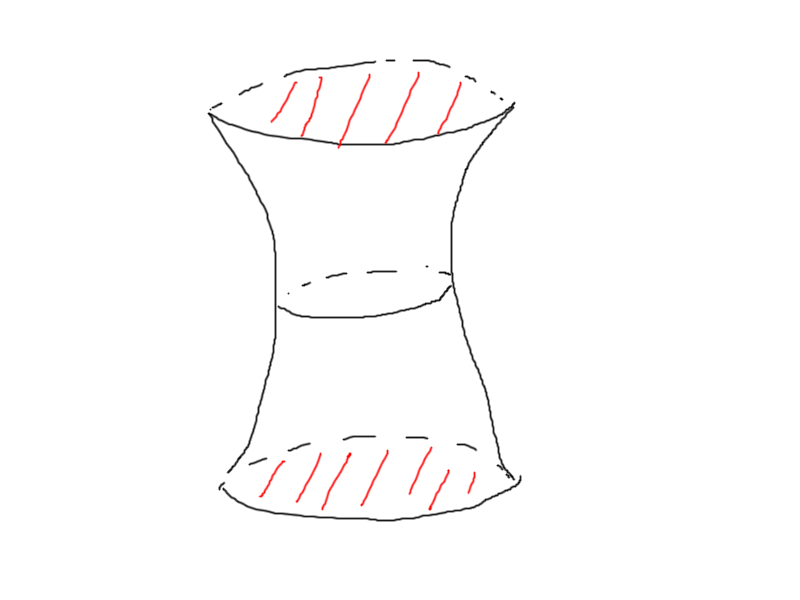
\includegraphics[width=0.7\textwidth]{felm_1soap.png}

\end{document}
